\documentclass[12pt]{article}

\usepackage{amsmath}
\usepackage{amssymb}
\usepackage{physics}
\usepackage{enumitem}
\usepackage{tikz}
\usetikzlibrary{arrows.meta,calc,decorations.pathmorphing}
\usepackage{geometry}
\geometry{margin=1in}

\begin{document}

\begin{center}
{\Large \textbf{SET 19 (Final Corrected Diagram-Validated Version)}}
\end{center}

\begin{enumerate}[leftmargin=*]

%====================================================
\item A small bead of mass $m$ slides without friction along a straight radial groove on a horizontal disc rotating with constant angular speed $\omega$. The bead is connected to the center by a spring of constant $k$ and natural length $l_0$. In the rotating frame, centrifugal force competes with spring restoring force and equilibrium shifts from $r=l_0$. After determining the new equilibrium radius and expanding the effective potential up to quadratic order, the condition for stable equilibrium is

\begin{center}
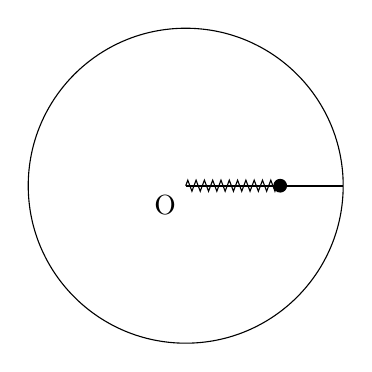
\begin{tikzpicture}[scale=1]
\draw (0,0) circle (2);
\draw[thick] (0,0) -- (2,0);
\draw[fill] (1.2,0) circle (0.08);
\draw[decorate,decoration={zigzag,segment length=3,amplitude=2}]
(0,0)--(1.2,0);
\node at (0,0) [below left] {O};
\end{tikzpicture}
\end{center}

\begin{enumerate}
\item $k > m\omega^2$
\item $k < m\omega^2$
\item $k = m\omega^2$
\item $k > 2m\omega^2$
\end{enumerate}

%====================================================
\item A particle moves in one-dimensional potential $V(x)=ax^4-bx^2$ with $a,b>0$. The system has two symmetric stable equilibria. After locating equilibrium positions and expanding the potential about one minimum to second order, the angular frequency of small oscillations is proportional to

\begin{enumerate}
\item $\sqrt{2b}$
\item $\sqrt{4b}$
\item $\sqrt{\dfrac{2b^2}{a}}$
\item $\sqrt{\dfrac{b^2}{a}}$
\end{enumerate}

%====================================================
\item An ideal gas is enclosed in a vertical cylinder of cross-sectional area $A$ with a movable piston of mass $M$. The piston is attached to a spring of constant $k$ and the system is thermally insulated. At equilibrium, pressure balances both weight and spring force. Let the equilibrium gas volume be $V_0$ and pressure be $P_0$. For a small vertical displacement, using adiabatic relation $PV^\gamma=\text{constant}$ and linearization of pressure change with volume, the angular frequency of small oscillations is

\begin{center}
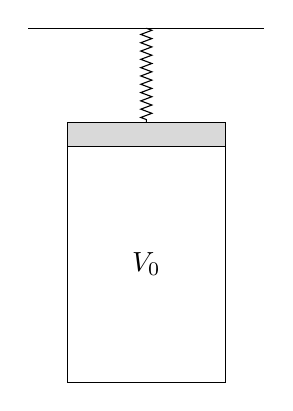
\begin{tikzpicture}[scale=1]
\draw (-0.5,4.5)--(2.5,4.5); % ceiling
\draw (0,0) rectangle (2,3);
\draw[fill=gray!30] (0,3) rectangle (2,3.3);
\draw[decorate,decoration={zigzag,segment length=3,amplitude=2}]
(1,4.5)--(1,3.3);
\node at (1,1.5) {$V_0$};
\end{tikzpicture}
\end{center}

\begin{enumerate}
\item $\sqrt{\dfrac{\gamma P_0 A^2/V_0 + k}{M}}$
\item $\sqrt{\dfrac{P_0 A^2 + k}{M}}$
\item $\sqrt{\dfrac{\gamma k}{M}}$
\item $\sqrt{\dfrac{\gamma P_0 A^2}{M}}$
\end{enumerate}

%====================================================
\item A uniformly charged solid sphere of radius $R$ and volume charge density $\rho$ contains a spherical cavity of radius $a$ whose center is displaced by vector $\vec{d}$ from the sphere center. Using superposition of two charge distributions and Gauss’s law, the electric field at the center of cavity is

\begin{center}
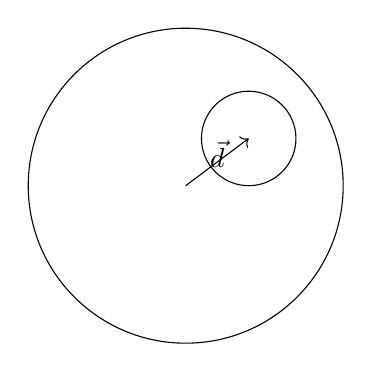
\begin{tikzpicture}[scale=1]
\draw (0,0) circle (2);
\draw (0.8,0.6) circle (0.6);
\draw[->] (0,0)--(0.8,0.6);
\node at (0.4,0.4) {$\vec d$};
\end{tikzpicture}
\end{center}

\begin{enumerate}
\item $\dfrac{\rho}{3\epsilon_0}\vec{d}$
\item $-\dfrac{\rho}{3\epsilon_0}\vec{d}$
\item $\dfrac{\rho}{\epsilon_0}\vec{d}$
\item $0$
\end{enumerate}

%====================================================
\item A parallel plate capacitor of area $A$ and separation $d$ is connected to a battery of voltage $V$. The plates are slowly pulled apart to separation $2d$ while battery remains connected. Considering change in capacitance, work done by battery, and field energy redistribution, the external work required is

\begin{enumerate}
\item $\dfrac{1}{4}CV^2$
\item $\dfrac{1}{2}CV^2$
\item $\dfrac{3}{4}CV^2$
\item $CV^2$
\end{enumerate}

%====================================================
\item An infinite ladder network consists of a resistor $R$ in series followed by a branch of two resistors $R$ in parallel, repeating indefinitely. Let equivalent resistance between input terminals be $R_{\text{eq}}$. Using self-consistency equation and solving resulting quadratic relation, the value of $R_{\text{eq}}$ is

\begin{enumerate}
\item $R(\sqrt{2}-1)$
\item $R(1+\sqrt{2})$
\item $R$
\item $\dfrac{R}{\sqrt{2}}$
\end{enumerate}

%====================================================
\item A charged particle enters crossed electric and magnetic fields such that initially $E=vB$ and it moves undeflected. The electric field is increased slightly to $E(1+\epsilon)$ where $\epsilon\ll1$. Using Lorentz force balance and first-order approximation, the fractional change in magnitude of net force on the particle is

\begin{center}
\begin{tikzpicture}[scale=1]
\draw[->] (-2,0)--(2,0) node[right] {$\vec v$};
\draw[->] (0,-2)--(0,2) node[above] {$\vec E$};
\foreach \x in {-1.2,0,1.2}
\foreach \y in {-1.2,0,1.2}
\node at (\x,\y) {$\otimes$};
\end{tikzpicture}
\end{center}

\begin{enumerate}
\item $\epsilon$
\item $-\epsilon$
\item $\dfrac{\epsilon}{2}$
\item $0$
\end{enumerate}

%====================================================
\item A long solenoid carrying steady current $I$ is stretched slowly so that its length increases and inductance decreases uniformly with time. Neglecting resistance and applying flux conservation, the induced emf at any instant is

\begin{center}
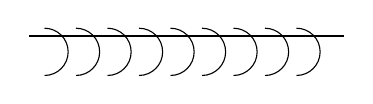
\begin{tikzpicture}[scale=1]
\draw[thick] (-2,0) -- (2,0);
\foreach \x in {-1.8,-1.4,...,1.8}
\draw (\x,-0.5) arc (-90:90:0.3);
\end{tikzpicture}
\end{center}

\begin{enumerate}
\item $-I\dfrac{dL}{dt}$
\item $-L\dfrac{dI}{dt}$
\item $0$
\item $\dfrac{d}{dt}(LI)$
\end{enumerate}

%====================================================
\item An inductive load draws current with lagging power factor $\cos\phi$. A capacitor is connected in parallel so that overall power factor becomes unity. Using phasor analysis and equating reactive powers, the required capacitive reactance $X_C$ is

\begin{enumerate}
\item $\dfrac{V^2}{Q}$
\item $\dfrac{Q}{V^2}$
\item $\dfrac{V}{Q}$
\item $QV$
\end{enumerate}

%====================================================
\item A thin convex lens of focal length $f$ is placed at distance $2f$ from a plane mirror. A point object is placed at distance $f$ in front of the lens. After first refraction, reflection from mirror, and second refraction through the lens, the final image position relative to object is determined by combined lens and mirror equations.

\begin{center}
\begin{tikzpicture}[scale=1]
\draw (-5,0)--(5,0);
\draw (0,-2)--(0,2);
\draw (4,-2)--(4,2);
\draw[fill] (-2,0) circle (0.08);

\draw[<->] (-2,-0.5)--(0,-0.5);
\node at (-1,-0.8) {$f$};

\draw[<->] (0,-0.5)--(4,-0.5);
\node at (2,-0.8) {$2f$};

\node at (0,2.2) {Lens};
\node at (4,2.2) {Mirror};
\end{tikzpicture}
\end{center}

The final image

\begin{enumerate}
\item coincides with object
\item forms at $2f$ from lens
\item forms at $f$ behind lens
\item forms at infinity
\end{enumerate}

%====================================================
\item Two coherent waves of amplitudes $a$ and $2a$ interfere at a point. An additional phase $\phi$ is introduced between them. If resultant intensity becomes equal to the mean intensity of the interference pattern, using full interference formula, the value of $\phi$ is

\begin{enumerate}
\item $\dfrac{\pi}{3}$
\item $\dfrac{\pi}{2}$
\item $\dfrac{2\pi}{3}$
\item $\pi$
\end{enumerate}

%====================================================
\item A radioactive nucleus $A$ decays to $B$ with decay constant $\lambda_1$, and $B$ decays to stable $C$ with constant $\lambda_2$. Initially only $A$ is present. By solving coupled differential equations and differentiating $N_B(t)$, the time at which $B$ is maximum is

\begin{enumerate}
\item $\dfrac{1}{\lambda_2-\lambda_1}\ln\left(\dfrac{\lambda_2}{\lambda_1}\right)$
\item $\dfrac{1}{\lambda_1}\ln\left(\dfrac{\lambda_2}{\lambda_1}\right)$
\item $\dfrac{1}{\lambda_2}\ln\left(\dfrac{\lambda_1}{\lambda_2}\right)$
\item $\dfrac{1}{\lambda_1-\lambda_2}$
\end{enumerate}

%====================================================
\item A photon of energy $E$ strikes a heavy stationary nucleus and produces an electron–positron pair. Using simultaneous conservation of energy and momentum and solving threshold condition, the minimum photon energy required is

\begin{enumerate}
\item $2mc^2$
\item $3mc^2$
\item $4mc^2$
\item $mc^2$
\end{enumerate}

%====================================================
\item A MOSFET operates in saturation with drain current $I_D=\frac{1}{2}k(V_{GS}-V_T)^2$. For small signal variation around operating point, transconductance $g_m=\dv{I_D}{V_{GS}}$. After linearization and evaluation at bias point, $g_m$ equals

\begin{enumerate}
\item $k(V_{GS}-V_T)$
\item $\dfrac{k}{2}(V_{GS}-V_T)$
\item $k(V_{GS}-V_T)^2$
\item $\dfrac{k}{2}(V_{GS}-V_T)^2$
\end{enumerate}

%====================================================
\item For an ideal gas, pressure $P=\frac{1}{3}\rho v_{\text{rms}}^2$. If rms speed increases by small fraction $\epsilon$, using first-order approximation, fractional change in pressure is

\begin{enumerate}
\item $2\epsilon$
\item $\epsilon$
\item $\dfrac{\epsilon}{2}$
\item $3\epsilon$
\end{enumerate}

\end{enumerate}

\end{document}
